%!TEX root = ../template.tex
%%%%%%%%%%%%%%%%%%%%%%%%%%%%%%%%%%%%%%%%%%%%%%%%%%%%%%%%%%%%%%%%%%%
%% chapter1.tex
%% NOVA thesis document file
%%
%% Chapter with introduction
%%%%%%%%%%%%%%%%%%%%%%%%%%%%%%%%%%%%%%%%%%%%%%%%%%%%%%%%%%%%%%%%%%%

\typeout{NT FILE chapter1.tex}%

\chapter{Introduction}
\label{cha:introduction}

%INTRO
\section{Motivation}
\label{sec:Motivation}

% Collision avoidance is a crucial element for any autonomous vehicle to gurantee safety. However the baseline framework of the usual online safety critical control techniques could have some limitations leading to suboptimal performance. In the context of space, the high budget missions along with the limited size to carry resources like fuel..., the recurrent spacecrafts maneuvers to avoid collisions with debris \cite{hall2014history} (and other hazards), lead essentially to a need for safety and reliability, but welcome to improved performance and possible costs reductions.  \par
% The \glsxtrfull{CLF-CBF} is a fast computationally control method that via quadratic optimisation problem, imposes safety and stability through the respective contraints. The technique lacks a prediction horizon as its decision is purely based on the given instant, driving the system close to the boundary which demands an high control inputs magnitude to maintain the system safe and if possible on track to the desired equilibrium point. However to ensure feasibility of the given optimisation problem, the stability objective is soften, potentially leading to deadlock situations and the system to undesired equilibrium close to the obstacle boundary. More than that, in the given formulation, the \glsxtrshort{CLF-CBF} show a lack of adaptability, a decrease in performance as the scenario differs from what was initially conceptualized. 

% It is a fundamental aspect of the operation of any autonomous vehicle to ensure collision avoidance, thus guaranteeing safety. Nevertheless,  the conventional online safety critical control techniques may exhibit certain limitations, resulting in suboptimal performance. In the context of space, in addition to the high-budget missions and the onboard limited resources (e.g. fuel), there is also the recurrent spacecraft manoeuvres to avoid collisions with debris~\cite{hall2014history}  (and other hazards). This results in a need for safety and reliability, but it also welcomes improved performance and possible cost reductions.  \par
% The \glsxtrfull{CLF-CBF} is a computational rapid control method that employs quadratic optimisation problems to impose safety and stability constraints. The technique lacks a prediction horizon, as the decision is based purely on the given instant. This results in the system coming close to the boundary, which demands high magnitude control inputs to maintain the system safe and, if possible, on track to the desired equilibrium point. Nevertheless, in order to guarantee the feasibility of the specified optimisation problem, the stability objective is relaxed, which may result in the system approaching an undesired equilibrium in the proximity to the obstacle boundary. Furthermore, the The \glsxtrshort{CLF-CBF} demonstrates an absence of adaptability and a decline in performance when confronted with scenarios that deviate from the original conceptualisation. 

Collision avoidance is a crucial element for any autonomous vehicle to gurantee safety.  Nevertheless,  the conventional online safety critical control techniques may exhibit certain limitations, resulting in suboptimal performance. \par

Safety has been a major topic with the constantly increasing intrusion of technology in society. And that have been gaining more and more relevance which can be seen since the introduction of roads, cars and trageddies that came along with it. In order to solve the problem there have been proposed solutions that encompass projecting better the roads, infracstructures and rules to control the traffic but specially minimize tragedies and deal better with dangerous human behaviour \cite{naumann2020systems}. Among the proposed solutions a well regarded one comes by implementing autonomous prevention systems such as speed enforcement contributing to cars but specially peoples safety \cite{seiler1998development, naumann2020systems}.\par

In space, there are factors that put spacecrafts safety in danger, namely, orbital debris around Earth and artificial satellites, among other hazards. Those factors can be difficult to predict and can damage the vehicle, or even compromise the operability of it, which results in increasing costs. Debris~\cite{hall2014history} can be categorized by its origin, mission-related operations, accidents, or intentional creation, with sizes varying up to the size of a tiny fleck of paint, but with the possibility of causing damage, since it can have relative speeds in LEO of 10 km/s. In 2013 there was an estimate that indicated that in that year the probability of a spacecraft and a space debris larger than 1cm colliding was around 50-67\% \cite{sorokin2013earth} per year and the probability has been increasing since then. Collisions with orbital debris or even active satellites have also a big responsibility to the generation of this amount of orbital debris. In 2009 the Iridium and Cosmos 2251 collide duplicating the chances of collision in \glsxtrshort{LEO} \cite{wright2010current} and the Briz-M explosion in 2012 contributing to that afterwards\cite{hall2014history}. Many of those fragments estimated to stay in orbit for thirty years \cite{wang2010analysis} unless there is a mission to clean it. \par 

If they are identified and dected in time then it is possible through a maneuver to keep the spacecraft safe, avoiding collision situations, which have happened inumerous times by the Space Shuttle and \glsxtrfull{ISS}. Between 1999 and around 2014, the \glsxtrshort{ISS} has done nineteen collision avoidance maneuvers, among them against debris from the Cosmos 2251 satellite \cite{hall2014history}. During avoidance maneuvres, it is expected to keep the spacecraft safe but it is also welcome to optimized performance, as they contribute to the already limited and not cheap fuel expenditure and also to satellites inactive for considerable periods. \par

Meanwhile, the high costs associated with the missions lead to greater supervision of the projects, which feeds into longer deadlines and an even greater need to try to achieve an even higher level of reliability through analyses and tests and, as can be seen in the final design of the products, to guarantee the maximum results of the project, which consequently results in even higher costs. In fact, the CubeSat Proximity Operations Demonstration \cite{spiegel2023cubesat} project due to bureaucratic, apparent problems with the propulsion systems and launch delays led to a seven-year delay, which meant  that the CubeSat would not be launched until 2022 with previous-generation hardware, but still with software improvements. Generally, some approaches are taken to try to reduce costs, such as in Research and Development, being common to opt for designs or even more archaic and highly researched techniques, which already have some confidence in terms of robustness, reliability and safety. According to \cite{wertz2011space} trends in the space industry, possibly to try to reduce costs, seem to be increasing the capacity of mission-related software in parallel with the evolution of processors, which are still limited in terms of computing power. \par

%-Falar que visto a pretensao seja nao ter humanos a bordo, com os delays de comunicasção entre a nave e ground station que se vira para a automação. Treminando que não ter eles a bordo agrega para menores custos devido ao facto de gastarem menos espaço, espaço esse lovre p+ara transportar recursos ou simplesmente reduzir o peso e gasto de combustivel, menos um salario e menos exposição aos efeitos contra os seres do planeta terra.
%In addition to improving the software, increasing automation on the vehicles is proving particularly relevant with advances in chip miniaturization and the considerable size occupied by human beings outside the needs to be had on board (limited size to resources, weight matters a lot, shielding to mitigate even more the effects on humans, exposition to harsh and danger conditions, salaries...), only gaining more strength with the desire to reduce the workload on the ground and the delays in communications that increase with the distance from the planet, making even more remote the possibility of controlling it manually from a base on the planet’s surface. The miniaturization of electronics goes hand in hand with the desire to make space more accessible, which is why work in the area such as [5](1ª parte do relatorio, primeira apresentação) aims to develop satellites on the scale of a chip at relatively low cost.

Radiation is a factor with major implications, posing high risks both for astronauts and for components such as the computers in aerospace vehicles that can suffer from single event effects \cite{label1996single}, so, solutions to mitigate the problem include increasing the shielding which it means adding more weight and costs, as well as adapting these processors to the space reality in order to combat the effect, an example of which is the self-correcting and low-cost RadPC-Lunar system \cite{major2021overview}. All that added to the already high costs from the respective mission reflects on lower power processors compared to the ones on the ground. Considering the limited resources on board, namely, the energy consumed by the processors and the processors reality, it is given preference for fast and computationally low control techniques. 

Therefore, there is a demand in low-effort control methods that garantee safety and are capable to achieve realiable techinques performance. Among the typical control techniques there is \glsxtrshort{LQR}, that is fast and consists in returning the optimal solution but of a linear and unconstrained problem, without garantees of safety. Another control method is \glsxtrshort{MPC} that solves a constrained open-loop discrete-time optimal control problem defined along an horizon at each sampling time, thus allowing the imposition of safety. From each of the optimizations results a sequence of control actions along the whole horizon, with generally the first one applied to the system. This method is characterized by providing optimal solutions of the given problem however with the cost of a high computation, specially if the system model is non-linear. Both of the methods already used in the \glsxtrshort{CPOD} space mission \cite{spiegel2023cubesat}, \glsxtrshort{LQR} for minor corrections during formation maintenence, \glsxtrshort{MPC} for ingress to a passively safe flying formation and Nonlinear-\glsxtrshort{MPC} was used for Near-Field Rendezvous (around tens of kilometres of distance) to compensate for less accurate predictions accumulated previously for greater distances. \par 

Meanwhile, the \glsxtrfull{CLF-CBF} is a computational rapid control method that employs quadratic optimisation problems to impose safety and stability constraints. The technique lacks a prediction horizon, as the decision is based purely on the given instant. This results in the system coming close to the boundary, which demands high magnitude control inputs to maintain the system safe and, if possible, on track to the desired equilibrium point. Nevertheless, in order to guarantee the feasibility of the specified optimisation problem, the stability objective is relaxed, which may result in the system approaching an undesired equilibrium in the proximity to the obstacle boundary. Furthermore, the \glsxtrshort{CLF-CBF} demonstrates an absence of adaptability and a decline in performance when confronted with scenarios that deviate from the original conceptualisation. 


\section{Literature Review}
\label{sec:Literature_Review}


Previously, one of the most used collision avoidance control techniques used to be \glsxtrfull{APF} \cite{krogh1984generalized, khatib1986real}, analogous to an energy and its gradient to a guiding force. A technique not that robust, subject to relatively highly sensible performance according to the environment and with high necessity to a fine tuning of its parameters. 

Meanwhile, it arises in popularity the \glsxtrfull{CBF} that allows to design a controller aiming to online, keep a system safe \cite{ames2019control}. It is characterized by a control affine constraint that, if respected, contributes to forward invariance of a well defined safe set. Compared to the \glsxtrshort{APF}, the \glsxtrfull{CBF} reveal more appetence, it generates smoother trajectories and is able to deal with more complex scenarios \cite{singletary2021comparative}.

The \glsxtrshort{CBF} is a generalization of the \glsxtrfull{CLF} \cite{sontag1983lyapunov, ames2014rapidly}, however during problems generally used as keep away behaviour from the unsafe states whilst \glsxtrshort{CLF} imposing an approximation to an equilibrium point, i.e, inducing asymptotically stability to an desired equilibrium state. 

Initially the \glsxtrshort{CBF} proposed in \cite{ames2014control} were unbounded near the boundary being propitious to numerical problems. Beyond that, there it was proposed a \glsxtrfull{QP} formulation, combining the \glsxtrshort{CLF} and \glsxtrshort{CBF} in order to synthesize a controller that could achieve safety and stability of the system, which is not always possible.  Afterwards, \cite{xu2015robustness} presented the zeroing \glsxtrfull{CBF} solving previous problem, taking null values at the boundary of the safe set and establishing it as the standard. Regarding the \glsxtrshort{QP}, more recently \cite{ames2019control} proposed a solution to ensure feasibility, by softening the stability objective, but potentially leading to deadlock situations.

%APRESENTAÇÃO

%This work, aims to generalize the the given algorithms to high-order systems, as robotic systems such as spacecrafts are generelly governed by high relative-degree constraints, therefore \cite{ames2019control} came with \glsxtrfull{ECBF} as a solution to it while \cite{taylor2022safe} with backstepping which was the chosen one to apply on this thesis experiments.

%Relevant to say, \glsxtrshort{CBF} have been gaining lots of focus in reasearch, including in spacecrafts and satellites \cite{breeden2022predictive, breeden2021guaranteed}, \glsxtrfull{UAV} \cite{matias2025hybrid, singletary2021comparative}, among many others robotic systems \cite{ames2019control} (bipedal robots, multi-robot systems...). 
% Previous articles purpose variations of the technique which lack adaptiveness as their parameters are constant and tuned according to a particular problem need/experiment. The proposed algorithms present an offline (or at least opportunistic) optimization of the severity of the \glsxtrshort{CBF} condition, making use of algorithms  such as gradient descent \cite{ruder2016overview}, highly used in deep learning \cite{tian2023recent}, or binary search \cite{lin2019binary}.  

%The techniques presented here are designed to be able to deal with unsafe sets graphically with different shapes and sizes, usually delimited by an ellipsoide but like \cite{matias2025hybrid}, is given the \glsxtrshort{CBF} formulation that enables encoding the obstacles complex shapes by doing the polytope fit shown in \cite{molnar2023composing}.   
% Like \cite{reis2020control, matias2025hybrid}, it is proposed a way to deal with undesired (asymptotically stable) equilibria in the closed-loop system, by changing the stabilization objective from the \glsxtrshort{CLF}, forcing the convergence of the closed-loop system to a point on the boundary of the safe set, but essentially aiming to optimize the path taken, relative to the nominal \glsxtrshort{CLF-CBF} framework. If is not capable to reach the desired state, through a \glsxtrshort{MPC}, sending the simulated trajectory as initial guess for a warm start optimization it is possible to mitigate the chances of a deadlock situation.

%EXTRAS

%The proposed techniques are compromised to deal with the respective characteristics. Among them the lack of adaptiveness through an offline (or at least opportunistic) optimization of the severity of the \glsxtrshort{CBF} condition, making use of algorithms  such as gradient descent \cite{ruder2016overview}, highly used in deep learning \cite{tian2023recent}, or a binary search \cite{lin2019binary} variation. There have been  Beyond that, it is proposed a way to deal with undesired (asymptotically stable) equilibria in the closed-loop system, by changing the stabilization objective from the \glsxtrshort{CLF}, forcing the convergence of the closed-loop system to a transitive deduced point on the boundary of the safe set, but essentially aiming to optimize the path taken, relative to the nominal \glsxtrshort{CLF-CBF} framework, avoiding the unwanted large inputs near the unsafe set while keeping the nominal speed of convergence. If it is not capable of reaching the desired state, through a \glsxtrshort{MPC}, sending the simulated trajectory as initial guess for a warm start optimization it is possible to mitigate even more the chances of a deadlock situation. 

%A \glsxtrshort{MPC} performs an optimization of multiple variables along an constrained receeding horizon (\glsxtrshort{MPC} applied in spacrafts rendezvous \cite{hartley2015tutorial, kaczmarek2023autonomous}), able to the incorporate \glsxtrshort{CBF} conditions to enforce safety of the close-loop system  \cite{grandia2021multi}, whilst \glsxtrshort{CLF-CBF} simply returns a single control input based on the given instant providing  faster computations.

%The aim of this thesis is develop a low-effort \glsxtrshort{CLF-CBF} based decision algorithm, suited to spacecrafts (processors), that similar to \cite{matias2025hybrid, reis2020control} comes by founding a closed-form solution of the constrained \glsxtrshort{QP}. The given solution is periodic but potentially being approximately continuous with the implementation of circuits designed to process gradient descent methods or even the closed-form solution of the respective \glsxtrshort{QP} \cite{hao2025analysis}.
The aim of this thesis is develop a low-effort \glsxtrshort{CLF-CBF} based decision algorithm, suited to spacecrafts (processors), that similar to \cite{matias2025hybrid, reis2020control} comes by founding a closed-form solution of the constrained \glsxtrshort{QP}. The controller is discrete, so the solution provided is periodic, but it is possible that it is approximately continuous with the implementation of circuits that have been designed to process gradient descent methods, or even the closed-form solution of the respective \glsxtrshort{QP}. \cite{hao2025analysis}.
\glsxtrshort{CLF-CBF} provides faster computations, but simply returns a single control input based on the given instant. In contrast, A \glsxtrshort{MPC} is a control method that performs optimisation of multiple variables along a constrained receding horizon. This subject has been extensively researched, including its application in the space industry (see, for example, \cite{hartley2015tutorial, kaczmarek2023autonomous}). \glsxtrshort{MPC} is able to incorporate \glsxtrshort{CBF} conditions to enforce the safety of a close-loop system \cite{grandia2021multi} along the whole horizon.

%This work aims to generalize the given algorithms to be able to deal with unsafe sets, usually delimited by an ellipsoide. Given the \glsxtrshort{CBF} formulation that enables encoding the obstacles complex shapes. \cite{molnar2023composing} presented a way to merge \glsxtrshort{CBF} via logical operations, providing a smooth approximation of the max and min functions representative of the AND OR operations.  
The objective of this work is to generalise the given algorithms so that they are able to deal with unsafe sets delimited by a non-ellipsoidal boundary, since the ellipsoidal fit is generally overconservative. \cite{molnar2023composing}  proposed a methodology for composing \glsxtrshort{CBF} via logical operations, thereby  providing a smooth approximation of the max and min functions, which are representative of the AND and OR operations, respectively.  

% The proposed techniques , also extends to high-order systems, as robotic systems such as spacecrafts are generally governed by high relative-degree constraints, therefore \cite{ames2019control} came with \glsxtrfull{ECBF} as a solution to it while \cite{taylor2022safe} adapted to context of \glsxtrshort{CBF} backstepping~\cite{sepulchre2012constructive} which was the chosen one to apply on this thesis experiments.
% Relevant to say, \glsxtrshort{CBF} have been gaining lots of focus in reasearch, including in spacecrafts and satellites \cite{breeden2022predictive, breeden2021guaranteed}, \glsxtrfull{UAV} \cite{singletary2021comparative}, among many others robotic systems \cite{ames2019control} (bipedal robots, multi-robot systems...). 
The proposed techniques , also extends to high-order systems, as robotic systems such as spacecrafts are generally governed by high relative-degree constraints, therefore \cite{ames2019control} came with \glsxtrfull{ECBF} as a solution to it while \cite{taylor2022safe} adapted to context of \glsxtrshort{CBF} backstepping~\cite{sepulchre2012constructive} which was the chosen one to apply on this thesis experiments.
Relevant to say, \glsxtrshort{CBF} have been gaining lots of focus in reasearch, including in spacecrafts and satellites \cite{breeden2022predictive, breeden2021guaranteed}, \glsxtrfull{UAV} \cite{singletary2021comparative}, among many others robotic systems \cite{ames2019control} (bipedal robots, multi-robot systems...). 

The proposed techniques are modified to address the issues described in the motivation. There is a lack of adaptiveness, which can be addressed through offline (or at least opportunistic) optimisation of the severity of the \glsxtrshort{CBF} condition. This can be achieved by employing algorithms such as gradient descent \cite{ruder2016overview}, which is widely utilised in deep learning \cite{tian2023recent}, or a binary search \cite{lin2019binary} variation.

% There have been ways proposed to address the problem \cite{braun2020comment, cortez2022compatibility}, between them, the \cite{reis2020control} presented a method as a way to deal with that, by composing a rotative \glsxtrshort{CLF} and adding to the \glsxtrshort{QP} formulation a \glsxtrshort{CBF} condition preventing the system convergence to the unwanted stabilization conditions related with the used \glsxtrshort{CLF}. Although the results don't show boundary equilibria, due to probably the \glsxtrshort{CLF} level set initial setup relative to the starting point the trajectories reveal undesired behaviours.
% Meanwhile, \cite{matias2025hybrid} presents a collision avoidance hybrid \glsxtrshort{CLF-CBF} framework given a polytopic delimitation of the unsafe states. Its method proposes as a solution a switching mechanism between active half-spaces and associated (intermediate) equilibrium points able to converge to the desired equilibrium point.
% Following a receeding horizon approach (like \glsxtrshort{MPC}), \cite{breeden2022predictive} formulates a \glsxtrshort{CBF} that under collision of a given nominal trajectory along the respective horizon, based on the supposing time until the next predicted collision and next local maximum of the \glsxtrshort{CBF} function is able to return a single control input preventing possible future collisions with minimal intrusion of the nominal controller.  

In addition, \cite{reis2020control}, demonstrated that the \glsxtrshort{QP} \cite{ames2019control} introduce undesired equilibrium points in the obstacles boundary and the conditions to that happen. A methodology has been proposed to deal with undesired (asymptotically stable) equilibria within the closed-loop system. This involves a modification of the stabilisation objective from the \glsxtrshort{CLF}, thereby compelling the convergence of the closed-loop system to a transitive deduced point on the boundary of the safe set. The primary objective is the optimisation of the trajectory taken, relative to the nominal \glsxtrshort{CLF-CBF} framework. This approach is intended to circumvent undesirable large inputs in the vicinity of the unsafe set, while maintaining the nominal speed of convergence. In the event that the system is unable to reach the desired state through the proposed techniques, through a \glsxtrshort{MPC} it is possible to mitigate the chances of a deadlock situation by sending the simulated trajectory as an initial guess for a warm start optimisation. 
In addressing the aforementioned problem, various approaches have been proposed~\cite{braun2020comment, cortez2022compatibility}. Among these, a methodology was proposed by \cite{reis2020control} to resolve the issue through the implementation of a rotary \glsxtrshort{CLF}. The \glsxtrshort{QP} formulation is augmented by a \glsxtrshort{CBF} condition that serves to prevent the system from converging to undesirable stabilisation conditions, associated with the employed \glsxtrshort{CLF}. Despite the absence of boundary equilibria, as evidenced by the \glsxtrshort{CLF} level set initial setup relative to the starting point, the trajectories manifest undesired behaviours. 
Meanwhile, \cite{matias2025hybrid} present a collision avoidance hybrid \glsxtrshort{CLF-CBF} framework given a polytopic delimitation of the unsafe states. The proposed methodology involves a switching mechanism between active half-spaces and associated (intermediate) equilibrium points, capable of converging towards the desired equilibrium point. 
Following a receding horizon approach (like \glsxtrshort{MPC}), \cite{breeden2022predictive}  propose a \glsxtrshort{CBF} that, in the event of a collision of a specified nominal trajectory along the designated horizon, is capable of returning a control input with the objective of preventing potential future collisions with a minimal interference of the nominal controller. This is based on the supposing time until the subsequent predicted collision and subsequent local maximum of the \glsxtrshort{CBF} function.  



%The proposed control techniques stand out by the fast computational speed, adaptatively capacity, options given the different scenarios and easy implementation. 

%ESTRUTURA
\section{Thesis Structure}
\label{sec:Thesis_Structure}

%This thesis starts in chapter \ref{cha:methodology} with the section \ref{sec:clf_cbf} by introducing the methodology of the \glsxtrshort{CLF-CBF}, including the formulation for backstepping, for the polytope fit and the closed-form controller governed by those concepts. Secondly, it is presented the particular methods used by the proposed techniques, the different single parameter optimization algorithms \ref{sec:Single_Parameter_Optmization}, such as variations of gradient descent and the binary search method, and coming after, is shown how to obtain the obstacle contour point \ref{sec:Constraint_Contour_Point}. Given the presented contents, in section \ref{sec:Proposed_Decision_Algorithms} it's elaborated the proposed algorithms. Finally, in chapter \ref{cha:results} there are simulations of the developed algorithms in collision scenarios, applied on a mixed-relative-degree-two unicycle system and on a second-order perturbed orbital model, both with their \glsxtrshort{CLF} and \glsxtrshort{CBF} defined accordingly. In the results it is provided the computational time of the respective algorithms and also some performance data. Concluding with chapter \ref{cha:conclusion}, providing some reflections on this thesis results and some suggestions on how to continue this work.
This thesis is structured as follows: the methodology of the CLF-CBF is introduced in section \ref{sec:clf_cbf}, including the formulation for backstepping, for the polytope fit and the closed-form controller able to deal with those concepts. Secondly, the dissertation proceeds to present the particular methods used by the proposed techniques, the different single parameter optimization algorithms (see section \ref{sec:Single_Parameter_Optmization}), such as variations of gradient descent and the binary search method. Following this, is shown how to obtain the obstacle contour point (see section \ref{sec:Constraint_Contour_Point}). In consideration of the preceding contents, the proposed control techniques are further elaborated in section \ref{sec:Proposed_Decision_Algorithms}. Finally, the results of the simulations of the developed algorithms are presented in Chapter \ref{cha:results} in different collision scenarios. These simulations were conducted on a mixed-relative-degree-two unicycle system and a second-order orbital model, with the \glsxtrshort{CLF} and \glsxtrshort{CBF} defined accordingly. The results section provides information regarding the computational time of the respective algorithms, in addition to certain performance data. The conclusion of this study is provided in Chapter \ref{cha:conclusion}, in which the results of the present research are reflected upon, and recommendations are made for the continuation of this work.































%Excertos de coisas que estavam no template versão original



%\prependtographicspath{{Chapters/Figures/Covers/}}

% epigraph configuration
%\epigraphfontsize{\small\itshape}
%\setlength\epigraphwidth{12.5cm}
%\setlength\epigraphrule{0pt}

%
\includegraphics[width=0.1\linewidth]{NOVAthesisFiles/Images/novathesis-insignia}\hfill
%
\includegraphics[width=0.875\linewidth]{NOVAthesisFiles/Images/novathesis-text}

% \noindent This is the \gls{novathesis} \LaTeX\ template \ntindex[Template!]{Version} \novathesisversion\ from   {Template!date}\novathesisdate.

% \epigraph{
%   This work is licensed under the \href{https://www.latex-project.org/lppl/lppl-1-3c/}{\LaTeX\ Project Public License v1.3c}.
%   To view a copy of this \ntindex[Template!]{license}, visit the \href{https://www.latex-project.org/lppl/}{LaTeX project public license}.
% }

% \section{Welcome to the \novathesis\ Template}
% \label{sec:if_you_use_this_template}

%~\ref{cha:users_manual}.

% \subsection{Your Time is Precious}
% \label{sub:time_is_money}

%\emph{learning the rules} 

%\begin{tcolorbox}[colback=green!8]
%\\\parbox{\linewidth}{\raggedleft---~\emph{João Lourenço}}
%\end{tcolorbox}

%\href{https://www.paypal.com/donate/?hosted_button_id=8WA8FRVMB78W8}{\fcolorbox{DarkGreen}{gray!15}{\textbf{~HERE~}}} 


% \begin{figure}[htbp]
%     \centering
%     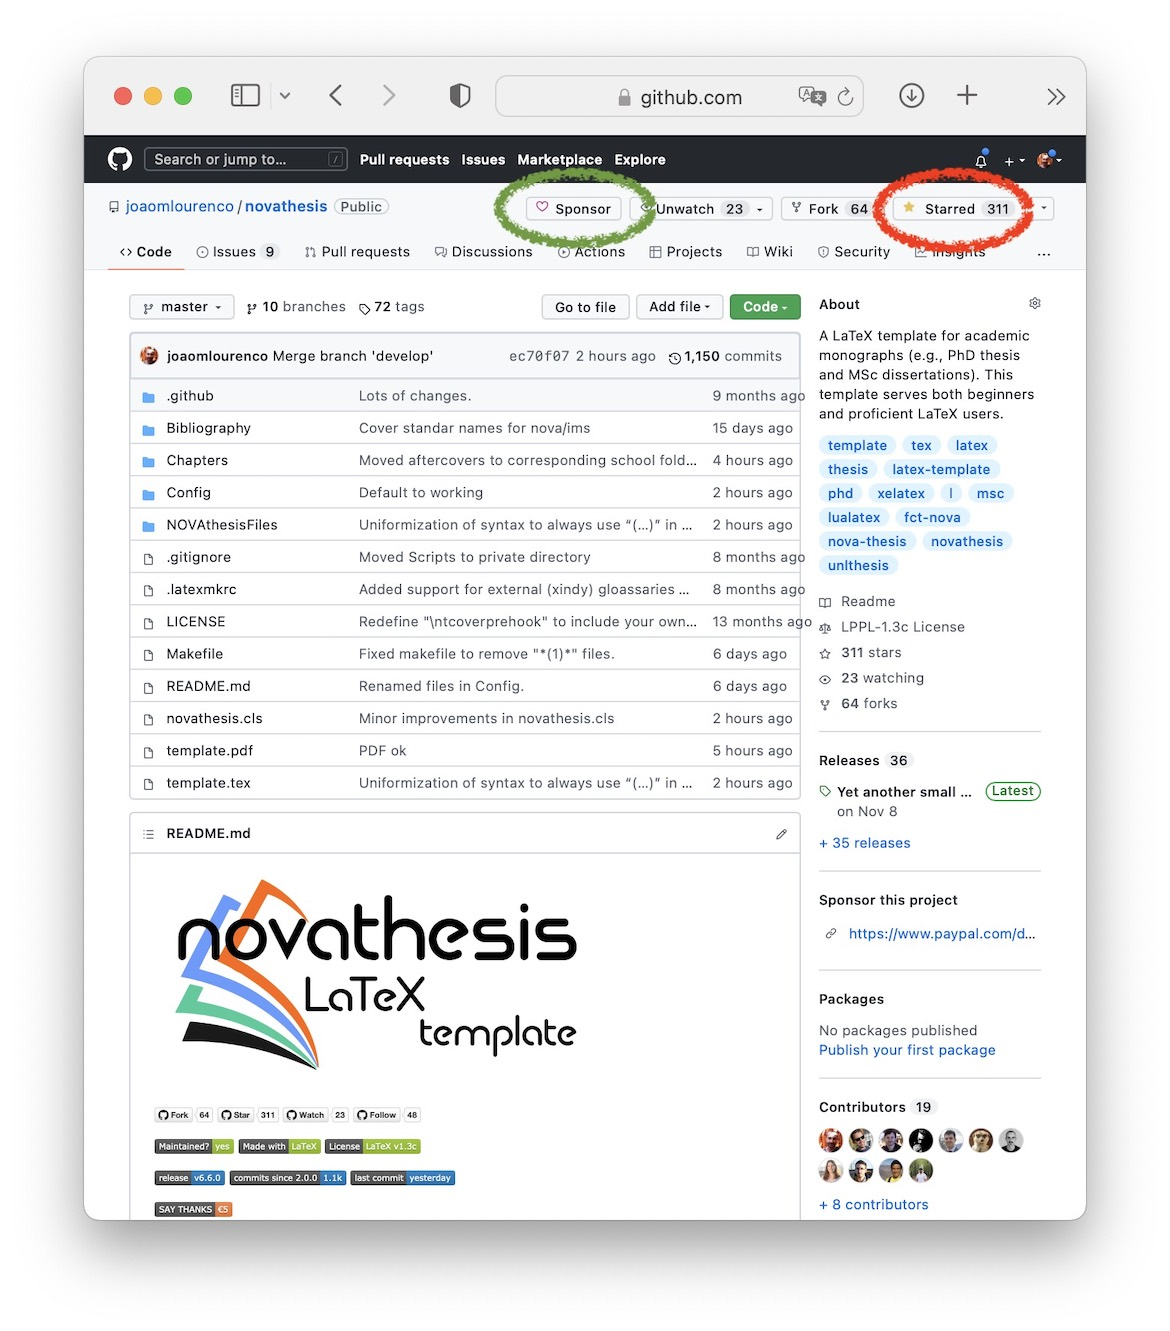
\includegraphics[width=0.5\linewidth]{github1}
%     \caption{The \gls{novathesis} project web page in GitHub.}
%     \label{fig:github}
% \end{figure}

% \section{The \emph{NOVAthesis} Template}
% \label{sec:a_bit_of_history}

% \ntindex[Template]{}

% \newenvironment{ntUniversity}[1]{
%   \renewcommand\tabularxcolumn[1]{m{##1}}% for vertical centering text in X column
%   % \renewcommand\cellgape{\Gape[1cm]}
%   % \setcellgapes{20pt}
%   % \makegapedcells
%   % % \setlength{\extrarowheight}{20pt}
%   % \renewcommand{\arraystretch}{2}
%   \rowcolors{1}{}{GhostWhite}
%     \xltabular{\linewidth}{cX}%
%       \caption{#1's Schools supported by the \gls{novathesis} template\label{tab:supported_schools_#1}}\\
%     \toprule%
%     \rowcolor{Gainsboro}%
%     & \Gape[1.5ex]{\thead[l]{#1}}\\
%     \midrule%
% }{%
%     \bottomrule
%     \endxltabular%
% }

% \makeatletter
% \newtoggle{coverspace}
% \newcommand{\docCover}[1]{%
%   \setlength{\fboxsep}{0pt}%
%   \togglefalse{coverspace}%
%     \Gape[1.5ex]{\begin{mcellbox}[cc]
%     \@for\myi:=#1\do{%
%       \fbox{\colorbox{White}{\includegraphics[align=c,width=1.5cm]{1up/\myi}}}%
%         \ifx\@xfor@nextelement\@nnil
%           % last iteration
%         \else
%           % not last iteration
%           \iftoggle{coverspace}{\togglefalse{coverspace}\\\\[-14pt]}{\toggletrue{coverspace}~}%
%         \fi
%   }%
%     \end{mcellbox}}
% }
% \makeatother
% \newcommand{\schlName}[3]{\textbf{#1} (\href{#3}{#2})}
% \newcommand{\degreeName}[3]{\newline\null\quad • #1 \href{#3}{(#2)}}

% \begin{ntUniversity}{NOVA University Lisbon}
%   {
%       \docCover{nova-fct-phd-en,nova-fct-msc-en}
%   } &  {
%     \schlName{NOVA School of Science and Technology}{FCT-NOVA}{https://www.fct.unl.pt}
%     \degreeName{All PhD Programs}{PhD}{https://www.fct.unl.pt/en/education/phd-programmes}
%     \degreeName{All MSc Programs}{MSc}{https://www.fct.unl.pt/en/education/master-degrees}
%   }\\
%   
% \end{ntUniversity}

% \newdata*{schlname}
% \newdata*{schlurl}
% \schlname(ea):={School of Architecture}
% \schlurl(ea):={https://www.uminho.pt/EN/uminho/Units/schools-and-institutes/Pages/School-of-Architecture.aspx}
% \schlname(ec):={School of Sciences}
% \schlurl(ec):={https://www.uminho.pt/EN/uminho/Units/schools-and-institutes/Pages/school-of-sciences.aspx}



% \subsection{Using Overleaf}
% \label{sub:using_overleaf}

% \ntindex[Installation!Overleaf]{}
% \ntindex[Using!Overleaf]{}

% \newcommand{\Overleaf}{\href{https://www.overleaf.com?r=f5160636&rm=d&rs=b}{Overleaf}}

% \begin{wrapfigure}{r}{0.3\linewidth}
% % \vspace*{-10ex}
% 
\includegraphics[width=\linewidth]{overleaf}%
% \caption{NOVAthesis template in Overleaf.}
% \label{fig:overleaf}
% \end{wrapfigure}
% \mbox{}\Overleaf\ is a collaborative cloud-based LaTeX editor used for writing, editing and publishing scientific documents. Like “Google Docs”,  

% \begin{tcolorbox}[colback=red!8]
% 	Notice that you need a (student) subscription to compile the \novathesis\ template in Overleaf, otherwise your compilation will always time out.
% \end{tcolorbox}

% \begin{description}
%   \item[Help:] If you just need some help, see above \Autoref{sec:getting_help}.
%   \item[Suggestion:] \ntindex[Suggestions]{} Do you have a suggestion/recommendation? Please add it to the wiki and help other users!
%   \item[Bug:] \ntindex[Bugs]{} Did you find a bug? Please open an issue. Thanks!
%   \item[New Feature:] \ntindex[Feature Requests]{} Would you like to request a new feature (or support of a new School)? Please open an issue. Thanks!

% \end{description}
